\def\year{2018}\relax
%File: formatting-instruction.tex
\documentclass[letterpaper]{article} %DO NOT CHANGE THIS
\usepackage{aaai18}  %Required
\usepackage{times}  %Required
\usepackage{helvet}  %Required
\usepackage{courier}  %Required
\usepackage{url}  %Required
\usepackage{graphicx}  %Required
\frenchspacing  %Required
\setlength{\pdfpagewidth}{8.5in}  %Required
\setlength{\pdfpageheight}{11in}  %Required
\copyrighttext{Copyright 2017, California Institute of Technology. 
Government sponsorship acknowledged.}
%PDF Info Is Required:
  \pdfinfo{
/Title (Extracting Information from Scientific Publications for
Planetary Science)
/Author (Kiri L. Wagstaff, Raymond Francis, Thamme Gowda, Nina L. Lanza,
You Lu, Ellen Riloff, Karanjeet Singh)}
\setcounter{secnumdepth}{0}  
 \begin{document}
% The file aaai.sty is the style file for AAAI Press 
% proceedings, working notes, and technical reports.
%
\title{Extracting Information from Scientific Publications for
Planetary Science}
\author{
Kiri L. Wagstaff$^1$,
Raymond Francis$^1$,
Thamme Gowda$^{1,2}$,
Nina L. Lanza$^3$,\\
{\Large \bf You Lu$^1$,
Ellen Riloff$^4$, and
Karanjeet Singh$^{1,5}$}\\
$^1$Jet Propulsion Laboratory, California Institute of Technology,
4800 Oak Grove Drive, Pasadena, CA 91109\\
\{firstname.lastname\}@jpl.nasa.gov\\
$^2$Information Sciences Institute, University of Southern
California,
4676 Admiralty Way \#1001, Marina Del Rey, CA 90292\\
tg@isi.edu
}
\maketitle
\begin{abstract}
We have constructed an information extraction system called the Mars
Target Encyclopedia that takes in planetary science publications
and extracts scientific knowledge.  The extracted knowledge is stored
in a searchable database that can greatly accelerate the ability of
scientists to compare new discoveries with what is already known.  To
date, we have applied this system to $\sim$6000 documents and achieved
XX\% precision in the extracted information. 
\end{abstract}

\section{Introduction}

Scientists everywhere are overwhelmed by the stream of new information
that is published by their disciplines' conferences, workshops, and
journals.  It is increasingly difficult to come up to speed in a
new area and to stay current with the latest discoveries.  In
planetary exploration, new discoveries can occur each time
new data is transmitted.  For example, our rovers on Mars have sent
back compositional data for thousands of individual targets (e.g.,
rocks, soils), and some of those observations have transformed our
understanding of past environments on the planet {\bf
[cite... Nature?]}.

To interpret new observations correctly, it is necessary to be able to
compare them with what is already known.  For example, if we observe
high manganese content at a particular location, we want to know
whether it is consistent with previous observations or it indicates an
anomalous new discovery.  However, no central database exists in which
planetary scientists can quickly make that determination.

We have created a system that uses information extraction methods to
analyze planetary science publications and identify compositional
relationships between Mars surface targets and elements or minerals.
The extracted information is stored in a searchable database that
allows users to ask questions such as ``Which targets contain
hematite?'' or ``What is known about target Dillinger?''  It also
enables entirely new kinds of information visualization, such as a map
display of all locations where the Mars rover Curiosity has detected
hematite. 

We focus on the extraction of information about targets identified by
the ChemCam instrument on the Mars Science Laboratory rover.  ChemCam
obtains compositional spectra from up to seven meters away from a
given target, and the resulting spectrum can be analyzed to identify
individual elements within the target~\cite{maurice:chemcam12}.  As of
sol 1159, ChemCam had observed more than 1100 distinct targets.

... provide guidance for next steps in exploration 
- hypothesis generation and data collection.

leveraged a small amount of hand-labeled text to train a

precision more important than recall

\section{Related Work}

GeoDeepDive

work at ISI?

\section{Machine Learning for Information Extraction}

The Mars Target Encyclopedia (MTE) is an information extraction system
that takes in scientific publications in PDF format and extracts
knowledge of use to planetary scientists studying the planet Mars.
The MTE is composed of four modules: preprocessing, named entity
recognition (NER), relation extraction (RE), and database updates (see
Figure~\ref{fig:mte}).

\begin{figure}
\begin{center}
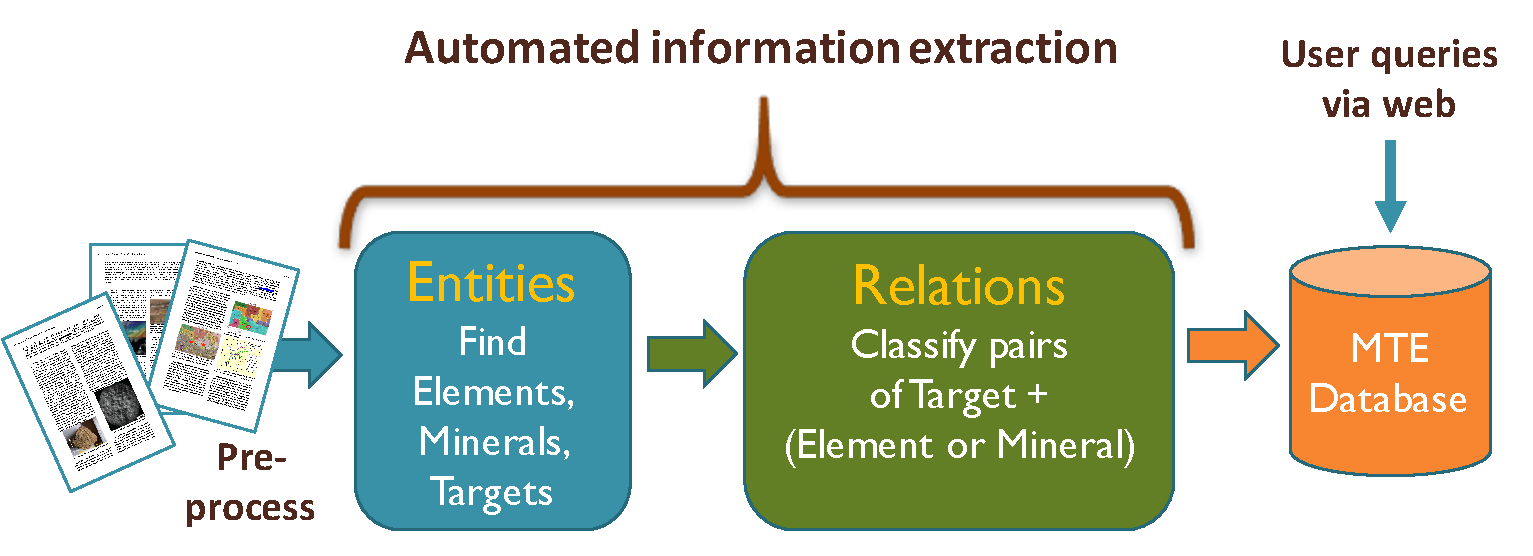
\includegraphics[width=3.25in]{fig/system.pdf}
\end{center}
\caption{Mars Target Encyclopedia processing pipeline.}
\label{fig:mte}
\end{figure}
% This figure comes from 2017-06-23-mte.pptx

\subsection{Document Preprocessing}

To prepare the documents for information extraction, the MTE first
extracts the text content from each PDF document.  We use the Apache
Tika parser~\cite{mattmann:tika11} to convert the source PDF files
into UTF-8 format text to preserve accented characters and
mathematical symbols.
% more details from extract_text_utf8.py?
Next, the MTE creates a copy of the text content in which the
References section is omitted.  We defined a regular expression to
identify the References section.
% show the regexp?
This step helps the NER component avoid spurious detections in the
titles or author names of cited publications.

\subsection{Named Entity Recognition}

The named entities of greatest relevance for the MTE are elements
(e.g., ``iron,'' ``Mg''), minerals (e.g., ``plagioclase,''
``hematite''), and ChemCam targets.  The periodic table provides a
comprehensive list of elements, and we employed a list of 5XXX minerals
provided by the International Mineralogical Association (from XXXX
2017, available at~\url{http://nrmima.nrm.se//imalist.htm}).

Identifying Mars surface targets is more challenging, as they follow
no standard naming convention.  Further, target names are
fundamentally ambiguous as they are borrowed from Earth locations or
people.  A sampling of the names hints at the challenge of accurately
detecting them: ``Dunkirk'', ``Ithaca'', ``Jake'', ``Old\_woman'',
``Pistol''.  We have a starting list of target names that was
published by the ChemCam science team, but we have found it to be
incomplete.  In addition, we found that authors invent new spelling
variants and abbreviations for target names that require more than a
simple list lookup.
% Keyword-based web or publication searches return many spurious hits.

To address the challenge of recognizing all three entity classes
reliably, we employed a machine learning approach.

- CoreNLP NER CRF
- gazettes - number of items in each (target, element, mineral)
- Basilisk~\cite{thelen:basilisk02}

{\bf [gazettes are available where online]}

\subsection{Relation Extraction}

- jSRE SVM

\section{Experimental Results}

We developed and evaluated the MTE using a collection of scientific
papers that were published over three years of the Lunar and Planetary
Science Conference (LPSC).

\subsection{Corpus}

Our corpus consists of two-page extended LPSC abstracts in PDF format.
We identified and manually annotated 117 documents from LPSC 2015 and
2016 that mentioned ``ChemCam.''  We used the brat annotation
tool~\cite{brat} to label entities and relations within these
documents.  We estimate that it took an average of 30 minutes to
annotate each document.  We created thousands of manual annotations in
62 documents from LPSC 2015 and 55 documents from LPSC 2016 (see
Table~\ref{tab:docs}).

We used the 2015 documents for training and divided the 2016 documents
for into validation ($n=20$) and testing ($n=32$) sets.

\begin{table}
\caption{Manual annotations for LPSC documents.}
\label{tab:docs}
\begin{center}
\begin{tabular}{l|ll}
Annotation & 2015 ($n=62$) & 2016 ($n=55$) \\ \hline
Element  & \\
Mineral  & \\
Target   & \\ \hline
Contains & \\ \hline
Total & \\
\hline
\end{tabular}
\end{center}
\end{table}

\begin{figure}
\begin{center}
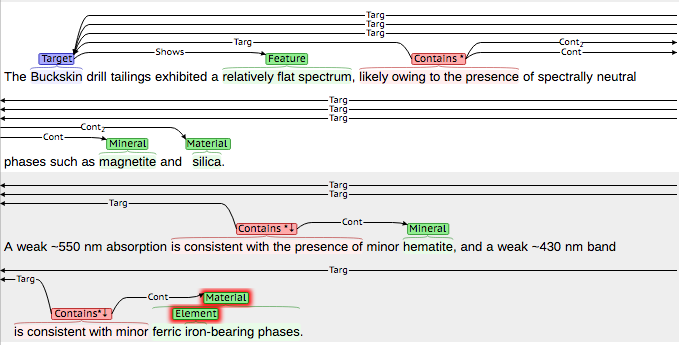
\includegraphics[width=3.25in]{fig/brat-example.png}
\end{center}
\caption{Excerpt from document lpsc16-1155 showing compositional
annotations created with the brat web annotation tool.}
\label{fig:brat}
\end{figure}

The annotated relationships ranged from simple (e.g., a pattern such
as ``X contains Y'' within a sentence) to complex (e.g., relationships
that crossed sentence boundaries or involved pronouns like ``it'' and
other anaphora).  Figure~\ref{fig:brat} shows an excerpt from one
document that contains several statements about the composition of the
target Buckskin.  The vocabulary used to indicate a compositional
relationship varies, and the last two relationships cross sentence
boundaries.  

{\bf [annotated docs are available where?]}

\subsection{Named Entity Recognition Results}

\begin{table}
\caption{Named entity recognition performance on LPSC 2016 test documents.  
The best result is shown in bold.}
\label{tab:ner}
\begin{center}
\begin{tabular}{l|ll}
 & Precision & Recall \\ \hline
Baseline: Lists only & P & R \\ \hline
{\em CoreNLP NER CRF trained on:} & & \\
LPSC 2015 & P & R \\
LPSC 2015 + gazettes & P & R \\
LPSC 2015 + Basilisk gazettes & P & R \\
\hline
\end{tabular}
\end{center}
\end{table}

{\bf [precision/recall per class - bar plot?]}

\subsection{Relation Extraction Results}

We created a training set using relations that were annotated in the
LPSC 2015 documents and a test set from relations in the LPSC 2016
documents.  We processed each sentence independently.  For each pair
of (Target, Element) or (Target, Mineral) within a sentence, we
generated a jSRE example that encoded the sentence content.  If the
pair of entities was connected by a relation in the manual
annotations, we gave the example a positive label; otherwise, we gave
it a negative label.

\begin{table}
\caption{Relation extraction performance on LPSC 2016 documents. 
The best result is shown in bold.}
\label{tab:re}
\begin{center}
\begin{tabular}{l|ll}
 & Precision & Recall \\ \hline
Baseline: All-yes & P & R \\ \hline
{\em jSRE SVM trained on:} & & \\
LPSC 2015, Target-Element & P & R \\
LPSC 2015, Target-Mineral & P & R \\
LPSC 2015, Target-Either  & P & R \\
\hline
\end{tabular}
\end{center}
\end{table}

[precision/recall per class - bar plot?]

\subsection{Large-scale Evaluation}

We collected all 6000 {\bf [check]} LPSC documents that were published
in 2014, 2015, and 2016 and ingested them into the MTE.  This large
corpus contains 117 manually labeled documents as well as everything
else that was published.

{\bf [table of num docs, num NER, num RE, time consumed]}

{\bf [Nina's evaluation of extracted information]}

\subsection{Limitations}
- NER cannot handle overlapping annotations (e.g., calcium sulfate)
- RE: no sentence-crossing relationships (about 30\%? recalc this number)

\section{Conclusions and Next Steps}
% and lessons learned

This work lies at the intersection of information extraction, machine
learning, and planetary science.  

% or is this a limitation (prev section)?
The MTE is not comprehensive.  There may be compositional information
that was never written up in a scientific publication and therefore
would not be included in the MTE.  Instead, the MTE extracts and
indexes only the information that was judged by scientists to be
worthy of publication to the scientific community.  The MTE leverages
and mirrors this selection bias, and its holdings (like the source
publications) contain only the most valuable and salient information.

We are in the process of integrating the MTE's content into the MSL
Analyst's Notebook, an interactive web resource for mission scientists
and the interested public.  The Analyst's Notebook allows users to
browse mission plans, targets discovered, data collected, and
summaries of each mission day on Mars.  The MTE content will enable
the Analyst's Notebook to also connect targets to publications.

Expand to targets identified by other missions such as the Mars
Exploration Rovers (Spirit and Opportunity).

\section{Acknowledgments}
This research was carried out in part at the Jet Propulsion Laboratory,
California Institute of Technology, under a contract with the National
Aeronautics and Space Administration.  {\bf [acks for Ellen, Nina?]}

\bibliography{mte}
\bibliographystyle{aaai}
\end{document}
